\chapter{ Hyperledger Fabric}
\label{chap:hyper}
\section{Giới thiệu Hyperledger Fabric }
Hyperledger Fabric là một nền tảng blockchain phân tán được phát triển bởi Linux. Nó 
cung cấp một giải pháp cho các tổ chức và doanh nghiệp để triển khai các ứng dụng blockchain 
tùy chỉnh. Hyperledger Fabric được thiết kế để có tính linh hoạt và khả năng mở rộng dễ dàng, 
cho phép các thành phần của hệ thống phát triển và triển khai độc lập với nhau.

Hyperledger Fabric có tính bảo mật cao và hỗ trợ quản lý danh tính và quản lý quyền truy cập, 
giúp bảo vệ dữ liệu của người dùng trên blockchain. Nó bao gồm các hợp đồng thông minh, sổ cái và
hệ thống mà người tham gia vào hệ thống quản lý các giao dịch của họ.


Điểm khác biệt giữa Hyperledger Fabric và các nền tảng blockchain khác là:
\begin{itemize}
    \item[-] Thiết kế dựa trên mô hình module 
    \item[-] Hỗ trợ quản lý danh tính và quyền truy cập
    \item[-] Độc lập với tiền tiện tử
    \item[-] Hỗ trợ các giao thức đồng thuận kết hợp
\end{itemize}

Fabric có kiến trúc linh hoạt, có thể thay đổi để đáp ứng cho nhiều lĩnh vực khác nhau, 
điều này chính là lý do em chọn Hyperledger Fabric để nghiên cứu và xây dựng ứng dụng.
\subsection{Mô hình mô-đun}

Hyperledger Fabric được thiết kế dựa trên mô hình mô-đun, cho phép các thành phần của hệ 
thống được phát triển và triển khai độc lập với nhau. Điều này giúp cho việc phát triển và 
triển khai các ứng dụng blockchain trở nên dễ dàng hơn.
Một Fabric tiêu chuẩn gồm các thành phần mô-đun sau:
\begin{itemize}
    \item[-] \textit{Dịch vụ đặt hàng (Ordering service)} được sử dụng để quản lý và xác nhận các giao dịch 
    trên mạng blockchain.
    
    \item[-] \textit{Dịch vụ cung cấp thành viên (Membership service provider)} là một thành phần trong hệ thống Hyperledger Fabric, 
    được sử dụng để quản lý và xác thực danh tính trên mạng blockchain. Nó đảm bảo rằng chỉ 
    các thành viên được ủy quyền mới có thể tham gia vào mạng blockchain và thực hiện các 
    hoạt động trên đó. MSP sử dụng các chứng chỉ xác thực để xác định quyền truy cập của mỗi thành viên trong mạng.
    \item[-] \textit{Dịch vụ nhắn tin ngang hàng (Cross-chain messaging service)} được sử dụng để cho phép các thành viên có thể 
    tương tác và giao tiếp với nhau trực tiếp, mà không cần thông qua một bên trung gian nào khác.
    \item[-] \textit{Hợp đồng thông minh (Chaincode)} chạy trong môi trường container như Docker. 
    Được viết bằng các ngôn ngữ lập trình để quy định các luật và điều khoản khi tham gia vào hệ thống. 
    \item[-] \textit{Sổ cái} nơi lưu trữ tất cả các thông tin về các giao dịch và trạng thái của mạng blockchain, 
    được hỗ trợ bởi nhiều hệ quản trị cơ sở dữ liệu.
    \item[-] \textit{Chính sách xác thực và chứng thực} có thể được thêm và áp dụng độc lập cho mỗi ứng dụng.
   
\end{itemize}

\subsection{Quản lý danh tính và quyền truy cập}

Hyperledger Fabric có tính năng hỗ trợ quản lý danh tính và quyền truy cập để đảm bảo 
tính bảo mật và phân quyền trong mạng blockchain. Dưới đây là một số tính năng quan trọng 
trong việc quản lý danh tính và quyền truy cập trong Hyperledger Fabric:

\begin{itemize}
    \item[-] Xác thực và ủy quyền: hỗ trợ nhiều phương thức xác thực và ủy quyền khác nhau, 
    chẳng hạn như xác thực bằng chứng chỉ SSL/TLS, xác thực bằng tài khoản và mật khẩu, 
    xác thực bằng access token và ủy quyền bằng các chứng chỉ.
    \item[-] Quản lý danh tính: cung cấp tính năng quản lý danh tính để quản lý các thông tin
    về người dùng và tổ chức trên mạng blockchain.
    \item[-] Quản lý quyền truy cập: cung cấp tính năng quản lý quyền truy cập để quản lý 
    người dùng đảm bảo rằng với mỗi người dùng có nhiệm vụ khác nhau thì quyền truy cập trong
    hệ thống là khác nhau.
    \item[-] Quản lý chứng chỉ: cung cấp tính năng quản lý chứng chỉ để quản lý các chứng chỉ
    và chứng thư số, để bảo mật và xác thực người dùng. \cite{hyperledger}

\end{itemize}
\subsection{Độc lập với tiền tiện tử}

Hyperledger Fabric là một nền tảng blockchain phổ biến được thiết kế để sử dụng trong các 
ứng dụng doanh nghiệp. Khác với các tiền điện tử như Bitcoin hay Ethereum, Hyperledger 
Fabric không phải là một loại tiền điện tử và không thực hiện các giao dịch tiền tệ. Thay 
vào đó, nó cung cấp các tính năng để đảm bảo tính toàn vẹn và bảo mật của dữ liệu trong 
mạng blockchain, giúp các doanh nghiệp triển khai các ứng dụng blockchain phù hợp với nhu 
cầu của họ.

Cụ thể hơn, trong Bitcoin hay Etherem, khi miner giải bài toán khó PoW để xác minh tính
toàn vẹn của thông tin sẽ được một phần thưởng là một lượng tiền điện tử. Thay vào đó, Hyperledger Fabric
sử dụng một hệ thống đồng thuận phân cấp để đảm bảo tính toàn vẹn và bảo mật của dữ liệu 
trên mạng blockchain. Các thành viên trong mạng Hyperledger Fabric được xác định và quản 
lý bởi các chứng chỉ xác thực và quy tắc thành viên. Khi một giao dịch mới được đề xuất, 
các thành viên trong mạng sẽ thẩm định và chấp nhận nó trước khi thêm vào blockchain.

\subsection{Cơ chế đồng thuận kết hợp}
Hyperledger Fabric là một nền tảng blockchain dành cho doanh nghiệp, có khả năng hỗ trợ 
nhiều cơ chế đồng thuận khác nhau như Proof of Work (PoW), Crash fault tolerant (CFT), Byzantine fault tolerant (BFT). Việc sử dụng cơ chế đồng thuận kết hợp trong 
Hyperledger Fabric được thực hiện nhằm đảm bảo tính toàn vẹn và bảo mật của hệ thống. 

Các cơ chế đồng thuận có thể được sử dụng tuỳ theo cài đặt của hệ thống. Mới mỗi hệ thống có 
số lượng thành viên tham gia và quy mô có thể lựa chọn cơ chế đồng thuận phù hợp với yêu cầu của hệ thống.

\section{Mô hình Hyperledger Fabric}
\subsection{Thành phần hệ thống}
\subsubsection{Nút}
Các nút trong hệ thống này đảm nhận các vai trò khác nhau. Mỗi loại nút có quyền truy cập và vai trò khác
nhau trong hệ thống.
Có 3 vai trò nút trong hệ thống:  
\begin{itemize}
    \item[-] Khách (Client): như là người dùng cuối, nó tạo và huỷ 
    các giao dịch, cho phép đảm nhận vai trò giao tiếp với các nút khác trong mạng.
    \item[-] Thành viên (Peer): Là nút mạng tham gia vào quá trình xử lý giao dịch và lưu trữ 
    dữ liệu trong mạng blockchain. Mỗi nút thành viên có một bản sao của sổ cái và có 
    thể thực hiện các chức năng như giao tiếp với các nút khác, đảm nhận xác thực và xử lý 
    giao dịch, thực hiện các chaincode (smart contract), cập nhật trạng thái của 
    sổ cái, và đồng bộ dữ liệu với các nút thành viên khác.
    
    Có hai loại nút thành viên khác nhau: người biểu quyết (Endorsers) và người xác thực (Committers).
        \begin{itemize}
            \item[+] Người biểu quyết: Mô phỏng, thực thi logic kinh doanh trong chaincode và xác minh tính hợp lệ giao dịch.
            \item[+] Người xác thực: Xác minh và xác nhận kết quả giao dịch trước khi thêm giao dịch vào blockchain. \cite{hyperledger1}
        \end{itemize}
    \item[-] Người đặt hàng (Orderer): vai trò là kênh liên lạc trung tâm cho mạng lưới, 
    đảm bảo các thành viên sẽ nhận chính 
    xác một thông điệp theo đúng logic và quản lý thứ tự của các 
    khối mới được thêm vào blockchain.
    
\end{itemize}
\subsubsection{Tài sản}
Tài sản là các đối tượng có giá trị được quản lý trên mạng blockchain trong 
Hyperledger Fabric. Mỗi tài sản có một ID duy nhất và được lưu trữ trong world state 
ledger. Trạng thái của mỗi tài sản được đại diện bởi cơ sở dữ liệu key-value và 
được cập nhật thông qua chaincode để tạo mới, cập nhật, xóa và truy vấn thông tin.
Các hoạt động này được thực hiện thông qua các giao dịch trên một Kênh.
\subsubsection{Chaincode}

Trong Hyperledger Fabric, hợp đồng thông minh được gọi là chaincode. Chaincode là 
một phần mềm các định một hoặc nhiều nội dung. Nó thực thi các quy tắc được xác định
để đọc và thay đổi các cặp giá trị key-value được lưu trữ trong sổ cái. 

Một giao dịch đề xuất thay đổi được gửi đến các nút thành viên trong mạng blockchain, và các 
thành viên thực thi chaincode để kiểm tra và xác minh giao dịch này. Nếu giao dịch thoả mãn các quy 
tắc được định nghĩa bởi chaincode, giao dịch sẽ được thực thi và kết 
quả được thêm cho sổ cái được lưu tất cả các nút thành viên.

\subsubsection{Sổ cái}
Mỗi sổ cái là một bản sao của toàn bộ blockchain và được lưu trữ trên mỗi nút thành viên trong mạng.
Hệ thống có thể lưu trữ nhiều sổ cái khác nhau, mỗi sổ cái được lưu trữ trên một channel riêng biệt. 
Trong Hyperledger Fabric, một sổ cái bao gồm 2 phần:

\begin{itemize}
    \item[-] World state ledger: Lưu trữ trạng thái hiện tại của tất cả các 
    tài sản trong mạng blockchain. World state ledger được lưu trữ dưới dạng cơ sở dữ liệu key-value, trong đó khóa là ID của tài sản và giá trị là trạng thái hiện tại của tài sản đó.
    \item[-] Transaction log ledger: Lưu trữ toàn bộ lịch sử các giao dịch được thực hiện 
    trên mạng blockchain. Transaction log ledger bao gồm các khối được kết nối theo đúng 
    thứ tự thời gian, mỗi khối chứa thông tin về các giao dịch được thực hiện trong khoảng 
    thời gian đó. Khác với World state ledger chỉ lưu trữ giá trị hiện tại, transaction log ledger
    lưu trữ toàn bộ lịch sử các giao dịch dưới dạng chuỗi các khối. Đây là
    một khối bất biến, không thể sửa đổi.
\end{itemize}
\subsubsection{Dịch vụ đặt hàng}
Nút đặt hàng thực hiện việc đặt hàng giao dịch, nút này 
cùng với các nút đặt hàng khác tạo thành một dịch vụ đặt hàng.
Dịch vụ đặt hàng cung cấp một kênh truyền thông cho 
các nút trong mạng để phát sóng các tin nhắn chứa các giao 
dịch, đồng bộ hoá các giao dịch và đảm bảo tính nhất quán 
của trạng thái blockchain.
Nút đặt hàng cũng thực thi kiểm soát truy cập cơ bản đối với 
các kênh, hạn chế người có thể đọc và ghi dữ liệu vào chúng 
cũng như ai có thể định cấu hình chúng. \cite{hyperledger1}

Khi khách hàng yêu cầu thêm một giao dịch trên blockchain, 
nó được đưa vào một gói tin và phát sóng đến Dịch vụ đặt 
hàng. Dịch vụ đặt hàng sẽ đảm bảo rằng các giao dịch được 
xử lý và đóng gói thành các khối theo một thứ tự nhất định 
và phát sóng đến tất cả các nút trong mạng. Các nút sau đó 
sẽ xác nhận và thêm khối này vào trạng thái blockchain của 
mình nếu khối đấy thoả mãn.

Trong dịch vụ đặt hàng sử dụng cơ chế đồng thuận Kafka Orderering Service (Kafka) để khi một 
khối mới được tạo ra bởi Kafka-based Ordering Service, nó sẽ được phát sóng đến tất cả các nút trong mạng. Các nút trong mạng sau đó sẽ xác nhận và kiểm tra tính hợp lệ của các giao dịch trong khối mới này.


\subsubsection{Kênh}

Trong hệ thống Hyperledger Fabric, kêng là một tính năng quan trọng để cung cấp cách thức 
truyền tải thông tin và giao tiếp bảo mật giữa các thành viên trong mạng blockchain.

Mỗi kênh là một nơi truyền thông riêng biệt giữa một nhóm các thành viên trong mạng, 
cho phép các thành viên trong kênh đóng vai trò như các bên liên quan duy nhất đến các giao 
dịch và trạng thái của sổ cái liên quan đến kênh đó. Điều này có nghĩa là nếu một thành 
viên không thuộc kênh không có quyền truy cập vào các giao dịch và trạng thái của kênh đó.

Mỗi kênh có một sổ cái riêng, bao gồm một World State Ledger và một Transaction Log Ledger, 
để lưu trữ thông tin về trạng thái hiện tại của tài sản trong sổ cái và lịch sử các giao dịch liên quan đến 
sổ cái đó. Khi một giao dịch được thực hiện trên một kênh, nó sẽ chỉ ảnh hưởng đến sổ cái 
của kênh đó và không ảnh hưởng đến các kênh khác.

Một thành viên có thể tham gia cùng lúc nhiều kênh và lưu trữ tất cả các sổ cái của các kênh.

\subsection{Cơ chế đồng thuận}

Đồng thuận là quá trình mà một mạng lưới các nút cung cấp thứ tự giao dịch được đảm 
bảo và xác thực khối giao dịch. Cơ chế đồng thuận cung cấp các chức năng chính sau: 

\begin{itemize}
    \item[-] Xác nhận tính chính xác của tất cả giao dịch trong một khối được đề xuất.
    \item[-] Đồng thuận về sổ cái giữa tất cả các nút thành viên.
    \item[-] Dùng hợp đồng thông minh để xác minh tính chính xác của từng giao dịch đã được sắp xếp trong một khối.
\end{itemize} 

Sự đồng thuận trong Hyperledger Fabric được chia làm 3 giai đoạn:

\begin{itemize}
    \item[-] Xác nhận: Nút thành viên có vai trò biểu quyết xác nhận giao dịch hợp lệ bằng cách ký chữ ký bảo lãnh.
    \item[-] Đặt hàng: Chấp nhận các giao dịch được xác nhận và đồng ý về thứ tự được thêm vào sổ cái.
    \item[-] Xác thực: kiểm tra một khối các giao dịch đã được sắp xếp và xác minh tính chính xác của kết quả, 
    bao gồm kiểm tra chính sách chứng thực và tránh tình trạng trùng lặp. \cite{consensus}
\end{itemize}

Cơ chế đồng thuận phủ khắp và bao gồm toàn bộ quá trình giao dịch. Các nút 
có nhiệm vụ khác nhau sẽ có vai trò khác nhau trong quá trình đồng thuận.

Hyperledger Fabric phiên bản v2.x đang sử dụng giao thức đồng thuận Raft để đảm bảo việc đồng thuận trong 
mạng blockchain. Raft là giao thức đồng thuận Crash fault tolerant - Khả năng chịu lỗi sự cố (CFT). 
Ví dụ như nếu có ba nút trong một kênh, nó có thể chịu được việc mất một nút (còn lại hai nút). 
Nếu bạn có năm nút trong một kênh, bạn có thể mất hai nút (để lại ba nút còn lại). 

\subsubsection{Thuật toán đồng thuận Raft}

Một cụm Raft bao gồm một số nút. Mỗi nút có thể ở một trong ba trạng thái: theo dõi, ứng cử viên hoặc 
lãnh đạo. Ban đầu các nút đều ở trạng thái theo dõi. Ở trạng thái này, họ có thể chấp nhận các mục nhật 
ký từ người lãnh đạo (nếu một người đã được bầu chọn) hoặc bỏ phiếu cho người lãnh đạo. Nếu không 
nhận được mục nhật ký từ người lãnh đạo hoặc người lãnh đạo mất kết nối nào trong một khoảng thời gian đã quy định, các nút sẽ chuyển thành 
trạng thái ứng cử viên. Ở trạng thái ứng cử viên, các nút yêu cầu phiếu bầu từ các nút khác. Nếu một 
ứng cử viên nhận được đủ số phiếu bầu, thì nút sẽ thành nút lãnh đạo. Người lãnh đạo phải chấp nhận 
các mục nhật ký mới và sao chép chúng cho những nút còn lại.


\subsection{Cấu trúc mạng Fabric}

Mạng Blockchain là một cơ sở hạ tầng kỹ thuật cung cấp sổ cái và hợp đồng thông minh (chaincode) cho các ứng dụng. 
Chaincode được sử dụng để tạo ra các giao dịch sau đó phân phối cho nút thành viên trong mạng. Người dùng ứng dụng
có thể là khách hàng hoặc quản trị viên của mạng blockchain.

Các tổ chức kết hợp với nhau để tạo thành một kênh trong đó các giao dịch được gọi 
trên chaincode và trong đó các quyền được xác định bởi một bộ chính sách được đồng ý 
khi kênh được định cấu hình ban đầu. Hơn nữa, các chính sách có thể thay đổi theo 
thời gian và phụ thuộc vào sự đồng ý của các tổ chức.

Đây là một ví dụ cấu trúc mạng cơ bản: 

\begin{figure}[h]
    \centering
    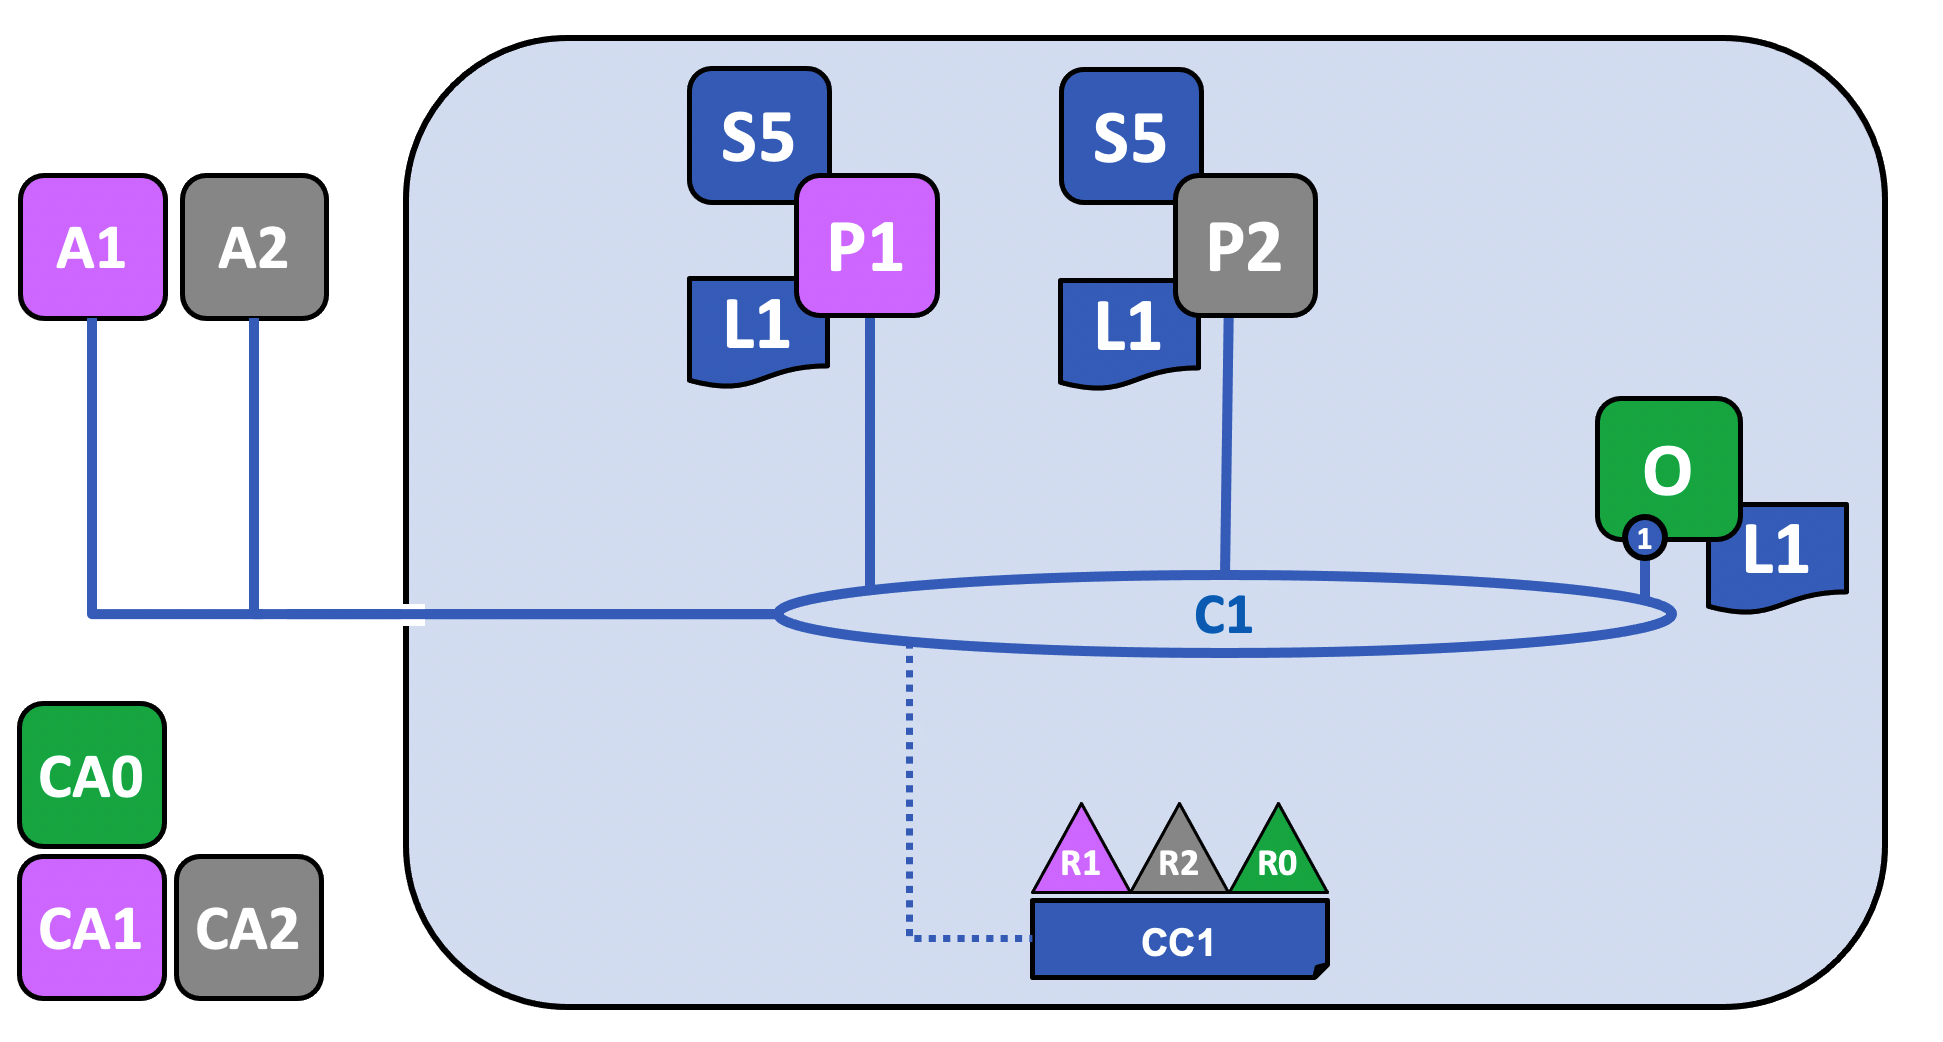
\includegraphics[width=0.9\textwidth]{images/network.png}
    \caption{Mạng Blockchain Hyperledger Fabric }
    \label{fig:network}
\end{figure}

Các thành phần trong mạng là:
\begin{itemize}
    \item[-] \textbf{CC:} Channel Configuration (Cấu hình của kênh).
    \item[-] \textbf{R:} Organization (Tổ chức).
    \item[-] \textbf{C:} Channel (Kênh), tập hợp các tổ chức có vai trò nhất định 
    trong cùng một quy trình kinh doanh. Ví dụ, trong một channel về mua bán 
    xe hơi sẽ gồm có 2 tổ chức là : Nhà sản xuất xe hơi, Nhà phân phối xe hơi.  
    \item[-] \textbf{P:} Peer (Nút thành viên) là điểm tương tác giữa các thành viên 
    trong tổ chức tương ứng với kênh, mọi hành động của người dùng đều 
    phải đi qua nó.
    \item[-] \textbf{O:} Orderer Node (Nút đặt hàng) tạo thành dịch vụ đặt hàng của kênh.
    \item[-] \textbf{L:} Ledger (Sổ cái) lưu trữ toàn bộ lịch sử giao dịch của kênh.
    \item[-] \textbf{A:} Application, ứng dụng hay giao diện (web, mobile app ) giúp người dùng tương tác với hệ thống dễ dàng hơn.
    \item[-] \textbf{CA:} Certificate Authority, phát hành danh tính cho người dùng 
    hoặc nút của tổ chức tương ứng. Ví dụ, người dùng A1 là thành viên của 
    Tổ chức R1, khi muốn tham gia vào mạng thì sẽ gửi yêu cầu đến CA1, 
    sau đó CA1 sẽ tạo ra một danh tính gồm khoá bí mật, khoá công khai và các 
    đặc tính liên quan khác, sau đó trả về cho người dùng A1, từ đó về sau 
    A1 dùng danh tính đó để thực hiện các tương tác với mạng, mạng sẽ tự động 
    biết đó là người dùng A1 đến từ tổ chức R1.
    \item[-] \textbf{S:} Smart Contract (Chaincode) được cài đặt trên kênh, định nghĩa rõ các hành động mà có thể thực hiện trên kênh.
    
\end{itemize}

Các bước để tạo một mạng Fabric:

\subsubsection{Tạo cơ sở mạng}

\begin{figure}[h]
    \centering
    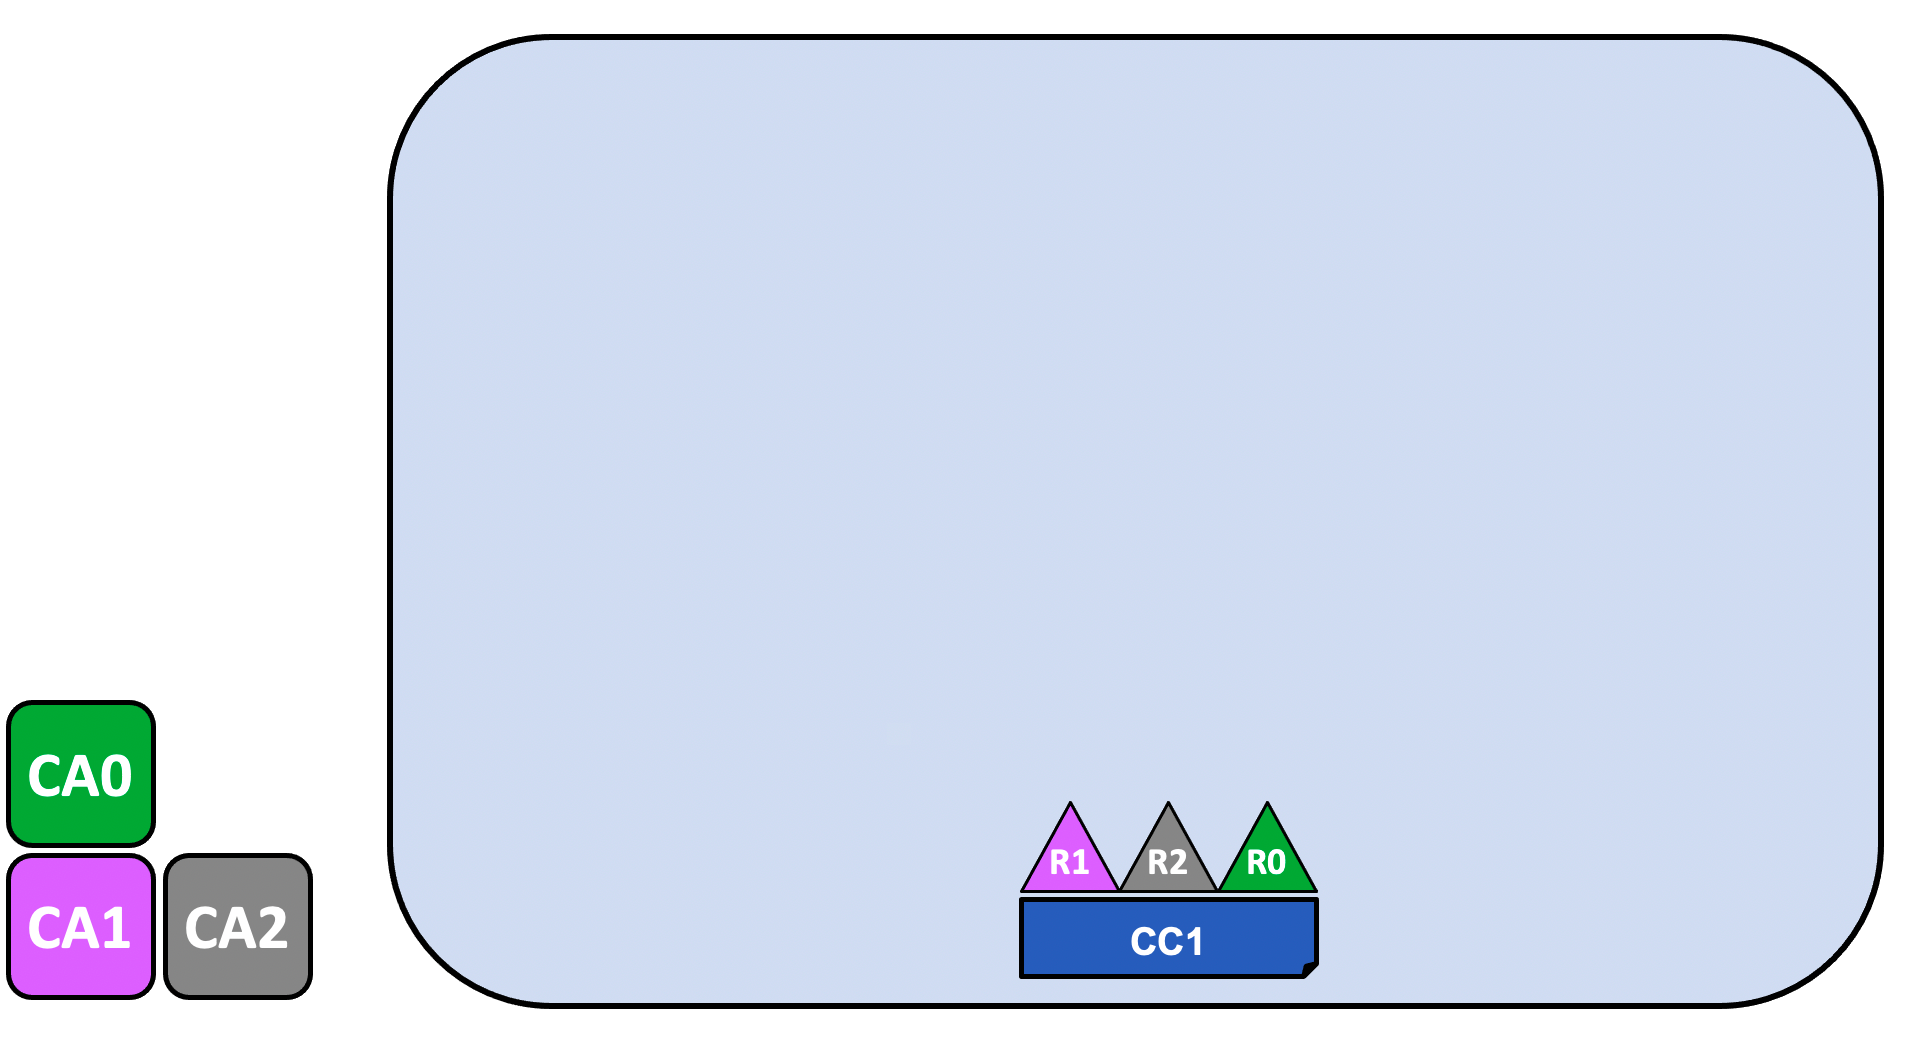
\includegraphics[width=0.8\textwidth]{images/create_network.png}
    \caption{Tạo mạng }
\end{figure}
Đầu tiên, các tổ chức R1, R2, R3 đồng ý sử dụng cấu hình CC1. Khối cấu hình được tạo. 
Khối cấu hình này chứa một bản ghi về các tổ chức có thể tham gia các thành phần và 
tương tác trên kênh, cũng như các chính sách xác định cấu trúc về cách đồng thuận để được các kết quả cụ thể.

Danh tính của các tổ chức này và danh tính của quản trị viên của họ phải 
được tạo bởi Tổ chức phát hành chứng chỉ (CA) được liên kết với từng tổ chức.

\subsubsection*{Tổ chức phát hành chứng chỉ (CA)}

Tổ chức phát hành chứng chỉ là một dịch vụ xác thực và quản lý chứng chỉ số trong hệ thống Hyperledger 
Fabric. Nó cung cấp các tính năng quản lý chứng chỉ số, chứng nhận, đăng ký và phân phối cho các thành 
phần trong mạng Hyperledger Fabric.

Các tính năng chính của CA bao gồm:

\begin{itemize}
    \item[-] Đăng ký danh tính cho các thành phần trong mạng: rootCert
    \item[-] Cấp giấy chứng nhận tuyển sinh (ECert): Khoá bí mật và công khai được tạo bởi ứng dụng khách Fabric CA, sau đó gửi khoá công khai
    đến CA để được trả về chứng chỉ.
    \item[-] Cấp, đổi, thu hồi chứng chỉ
\end{itemize}



Các thành phần khác nhau của blockchain sử dụng các chứng 
chỉ để xác định lẫn nhau là từ một tổ chức cụ thể. Ở ví dụ tạo mạng trên, 
ta có 3 CA đại điện cho 3 tổ chức.


CA tạo danh tính bằng cách tạo khóa công khai và khóa riêng tạo thành một cặp khóa có thể được sử dụng 
để chứng minh danh tính. Để xác định danh tính, ta phải cần một cơ quan đáng tin cậy đó là Nhà cung cấp dịch vụ thành viên (MSP).

MSP là một tập hợp các thư mục được thêm vào cấu hình mạng của kênh và được sử dụng để xác định 
quyền thực thi của tổ chức. MSP chứa danh sách danh tính được chấp nhận trong kênh, chức 
vụ và xác định quyền cho một nút trên kênh. 


\subsubsection{Các nút tham gia vào kênh}

\begin{figure}[h]
    \centering
    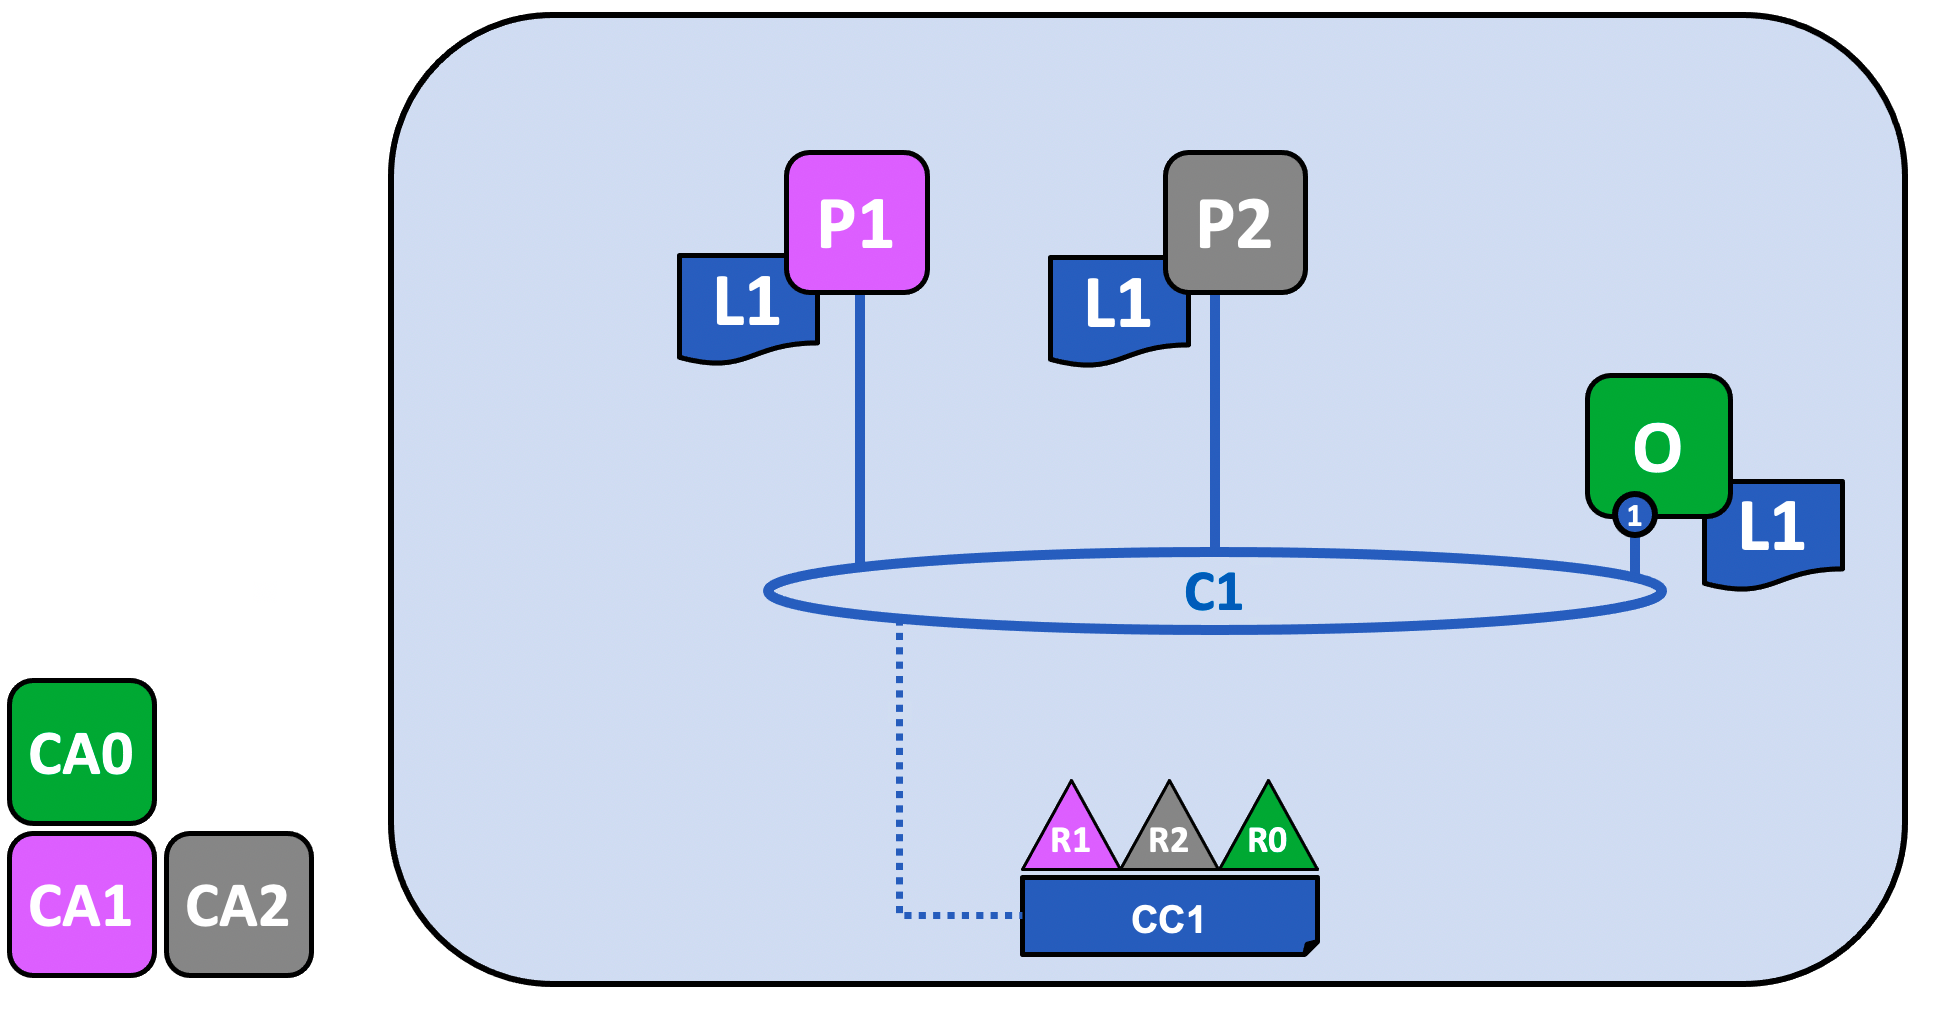
\includegraphics[width=0.9\textwidth]{images/join_network.png}
    \caption{Các nút tham gia vào kênh }
\end{figure}

Các nút thành viên, đặt hàng tham gia vào kênh. Các nút thuộc về mỗi tổ chức có chứng chỉ x.509 do Cơ quan cấp chứng chỉ 
liên kết với tổ chức đó tạo cho chúng. Chứng chỉ của P1 được tạo bởi CA1, chứng chỉ của P2 được tạo 
bởi CA2, v.v.

\subsubsection{Cài đặt và khởi tạo chaincode}

Chaincode được cài đặt trên các nút thành viên, sau đó được khởi tạo trên kênh. 

\begin{figure}[h]
    \centering
    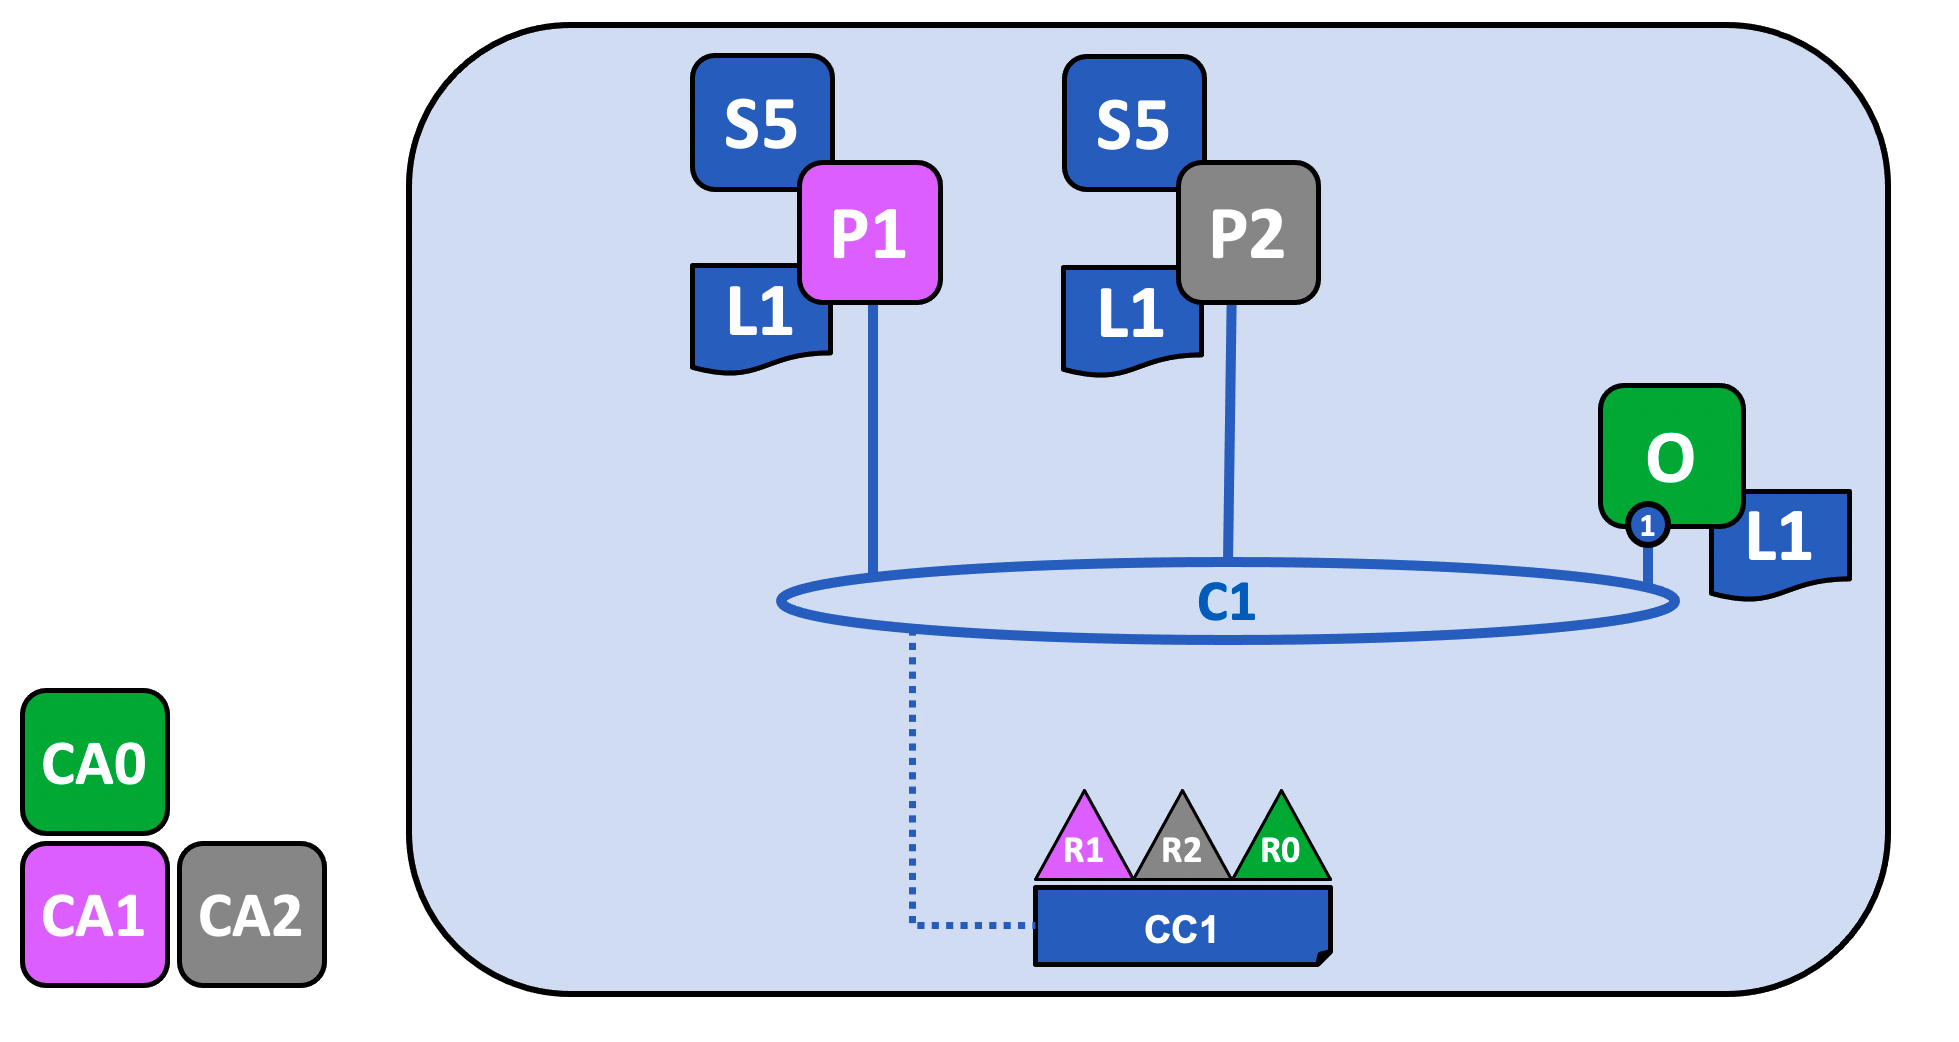
\includegraphics[width=0.9\textwidth]{images/install_chaincode.png}
    \caption{Cài đặt và khởi tạo chaincode}
\end{figure}

\subsubsection{Thêm ứng dụng khách trên kênh}

Sau khi hợp đồng thông minh đã được cam kết, các ứng dụng khách có thể được sử dụng để gọi 
các giao dịch thông qua các hàm chaincode. Sau bước này, mạng đã sẵn sàng để sử dụng.
Mạng được tạo sẽ có cấu trúc như hình \ref{fig:network}.

\subsection{Luồng giao dịch}
\label{subsec:luonggiaodich}
Luồng giao dịch có các bước sau:
\begin{figure}[h]
    \centering
    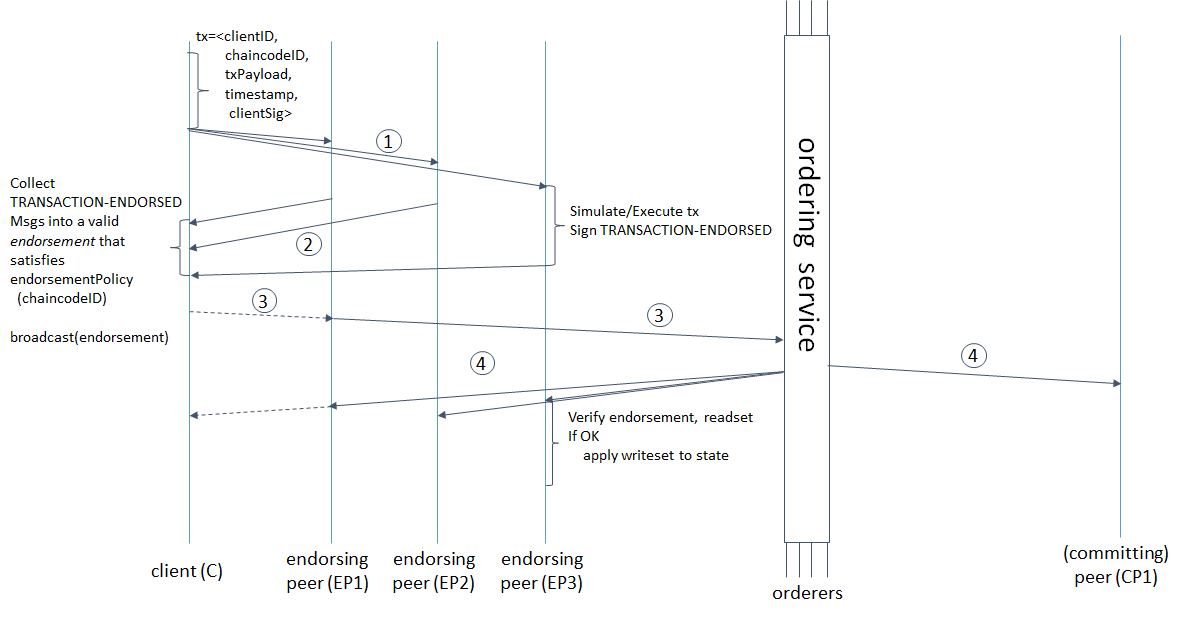
\includegraphics[width=1\textwidth]{images/flow-4.png}
    \caption{Luồng giao dịch }
\end{figure}


\begin{itemize}
    \item[\textbf{1.}] Khách gửi một giao dịch đến các  nút biểu quyết. Nút biểu quyết được sử dụng để chứng nhận tính hợp 
    lệ của một giao dịch trước khi nó được gửi đến các nút khác để xác nhận và cam kết trên 
    sổ cái. Nó không lưu trữ trực tiếp các thông tin liên quan đến giao dịch hoặc sổ cái.
    \item[\textbf{2.}] Khi một giao dịch được gửi đến nút biểu quyết, nó sẽ thực hiện một số hoạt 
    động để chứng nhận tính hợp lệ của giao dịch đó. Đầu tiên, nó sẽ kiểm 
    tra giao dịch này đã từng được gửi hay chưa để đảm bảo không trùng lặp. Chaincode sẽ được thực thi
    và trả về kết quả. Với mỗi một lệnh được thực hiện thì ta ghi lại 
    trạng thái đọc và ghi của dữ liệu, gọi là tập ReadWrite (RW).
    Nếu nút này thấy là giao dịch hợp lệ, nó sẽ tạo một chữ ký bảo lãnh. Tập RW cùng chữ ký sẽ được gửi lại cho người 
    gửi giao dịch. 
    \item[\textbf{3.}] Khi một giao dịch được ký chữ ký bảo lãnh, khách sẽ gửi giao dịch
    đó đến các ordering service. Người đặt hàng sẽ xác định thứ tự của các khối dựa trên 
    chữ ký bảo lãnh của nút biểu quyết và sắp xếp các giao dịch vào các khối tương 
    ứng. Sau đó nó gửi các khối đến toàn bộ nút thành viên.
    \item[\textbf{4.}] Người xác thực kiểm tra lại chính sách xác thực và kiểm tra hiệu lực của tập RW. Việc xác nhận giao dịch sẽ được lưu vào World- state, còn sổ cái sẽ lưu lại các giao dịch. 
    Khối sẽ được đánh dấu là hợp lệ hoặc không hợp lệ.
    \item[\textbf{5.}] Nếu khối là hợp lệ. Khối sẽ được thêm vào chuỗi. Các nút thành viên cập nhật lại trạng thái của sổ cái theo giao thức đồng thuận Raft.
    Thông báo lại kết quả cho ứng dụng khách. \cite{hyperledger}
\end{itemize}
